% No New page; first instance
\visHeader
\subsection[The visual language definition: Modeling with Diagrams]{The visual language definition; Modeling with \mbox{Enterprise Architect}}
\label{sec:staticAbstract}

\vspace{0.5cm}

\hypertarget{static vis}{You can begin modeling Leitner's Box in one of two ways} - You can build the diagrams in the same workspace as the Part I demo by opening the old \texttt{`demo.eap'} file, or you can start afresh by going to ``New Metamodel Project,'' choosing to start a new visual project without a demo (Fig.~\ref{fig:new_visModel}), and opening that \texttt{.eap} file. This handbook has assumed you prefer the latter, which is reflected only in the screenshots. If you use the previous files, please note that the steps are exactly the same, but our package explorers may not match exactly. Keep a sharp eye out for footnotes which explain the few differences.

\begin{figure}[htbp]
	\centering
  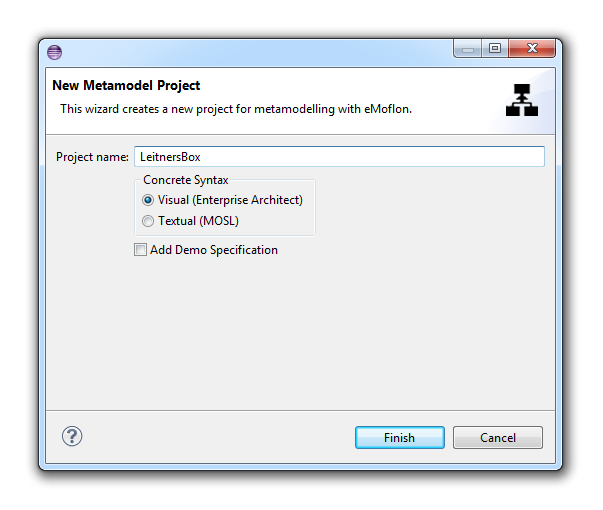
\includegraphics[width=0.7\textwidth]{eclipse_newMetamodelVisualPlain}
	\caption{Starting a new visual project}
	\label{fig:new_visModel}
\end{figure}
\begin{itemize}

\item[$\blacktriangleright$] From EA, select your working set and click on the \texttt{Add a Package} button (Fig.~\ref{fig:new_package}).

\begin{figure}[htbp]
	\centering
  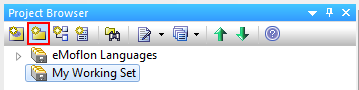
\includegraphics[width=0.5\textwidth]{ea_addPackage}
	\caption{Add a new package to \texttt{Demo}.}
	\label{fig:new_package}
\end{figure}



\item[$\blacktriangleright$] In the dialogue that pops up (Fig.~\ref{fig:new_package_name}), choose \texttt{Class View}, enter \texttt{Learning\-Box\-Language} as the name of the new package and click \texttt{OK}.

\begin{figure}[htbp]
	\centering
    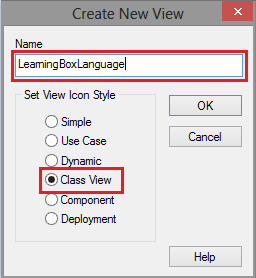
\includegraphics[width=0.33\textwidth]{EA_namePackage.png}
	\caption{Enter the name of the new package.}
	\label{fig:new_package_name}
\end{figure}
\FloatBarrier


\vspace{0.5cm}
\item[$\blacktriangleright$] Your \texttt{Project Browser} should now resemble figure~\ref{fig:new_package_completed}.

\begin{figure}[htbp]
	\centering
  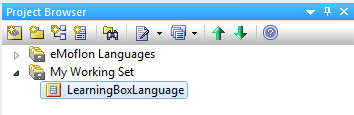
\includegraphics[width=0.6\textwidth]{ea_newPackage}
	\caption{State after creating the new package.}
	\label{fig:new_package_completed}
\end{figure}
\FloatBarrier



\item[$\blacktriangleright$] Now create a \texttt{New Diagram} (Fig.~\ref{fig:diagram}).

\vspace{0.5cm}

\begin{figure}[htbp]
	\centering
  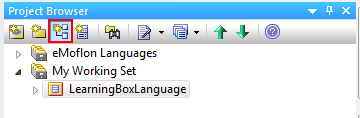
\includegraphics[width=0.6\textwidth]{ea_addDiagram}
	\caption{Add a diagram.}
	\label{fig:diagram}
\end{figure}
\FloatBarrier



\item[$\blacktriangleright$] In the dialogue that appears, (Fig.~\ref{fig:diagram_type}), choose \texttt{eMoflon Ecore Diagrams}, then select \texttt{OK}.

\end{itemize}

\pagebreak

\begin{figure}[htbp]
	\centering
  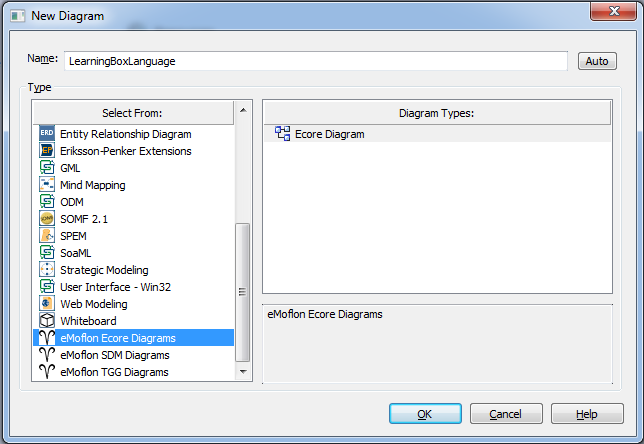
\includegraphics[width=0.8\textwidth]{EA_chooseDiagramType}
	\caption{Select the ecore diagram type}
	\label{fig:diagram_type}
\end{figure}
\FloatBarrier

\begin{itemize}
 
\item[$\blacktriangleright$] After creating the new diagram, your  \texttt{Project Browser} should now resemble figure~\ref{fig:diagram_completed}.

\begin{figure}[htbp]
	\centering
  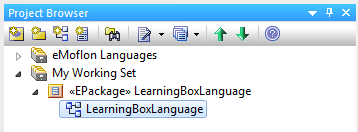
\includegraphics[width=0.6\textwidth]{ea_afterDiagramState}
	\caption{State after creating diagram}
	\label{fig:diagram_completed}
\end{figure}


\item[$\blacktriangleright$] Double-click the newly created diagram to ensure that it is open.


\item[$\blacktriangleright$] To the left of the workbench in EA, a \emph{Toolbox} containing the types available in Ecore for metamodelling should have appeared\footnote{If not, choose ``Diagram/Diagram Toolbox'' to show the current toolbox.}(Fig.~\ref{fig:eclass}). Click on \texttt{EClass}, then click in the open diagram. Alternatively, you can `drag-and-drop' the small eclass icon into the diagram window.

\begin{figure}[htbp]
	\centering
  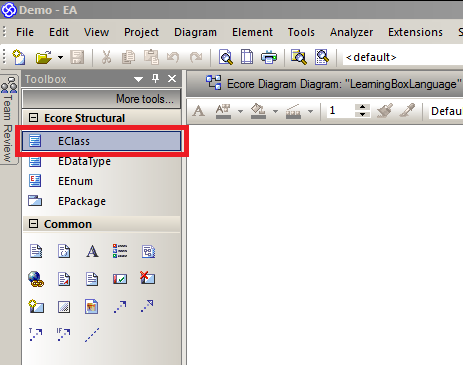
\includegraphics[width=0.7\textwidth]{EA_createEClass}
	\caption{Create an EClass}
	\label{fig:eclass}
\end{figure}



\item[$\blacktriangleright$] In the dialogue that pops-up, enter \texttt{Box} as the name of the class and click \texttt{OK} (Fig.~\ref{fig:eclass_properties}).
This dialogue can always be invoked by double-clicking the class, and contains many other properties we'll look into later in the handbook.
In general, a similar ``properties'' dialogue can be opened in the same fashion for almost every element in EA.

\begin{figure}[htbp]
	\centering
  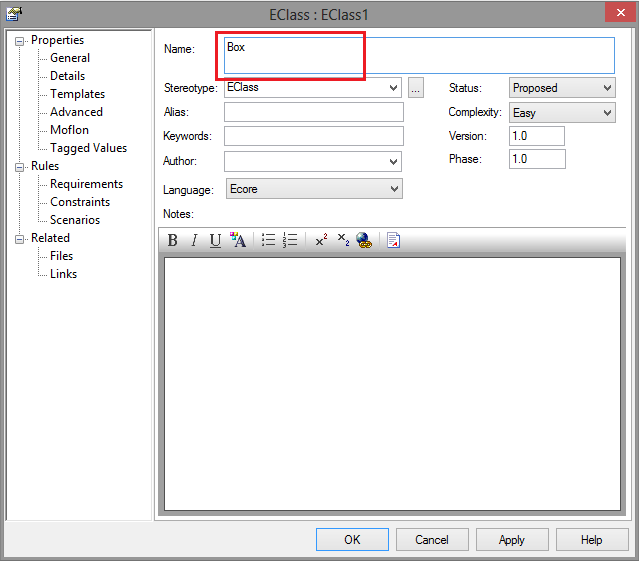
\includegraphics[width=0.6\textwidth]{EA_propertiesEClass}
	\caption{Enter properties of EClass}
	\label{fig:eclass_properties}
\end{figure}

\vfill
\pagebreak

\item[$\blacktriangleright$] After creating \texttt{Box}, your EA workspace should resemble figure~\ref{fig:eclass_completed}.

\begin{figure}[htbp]
	\centering
  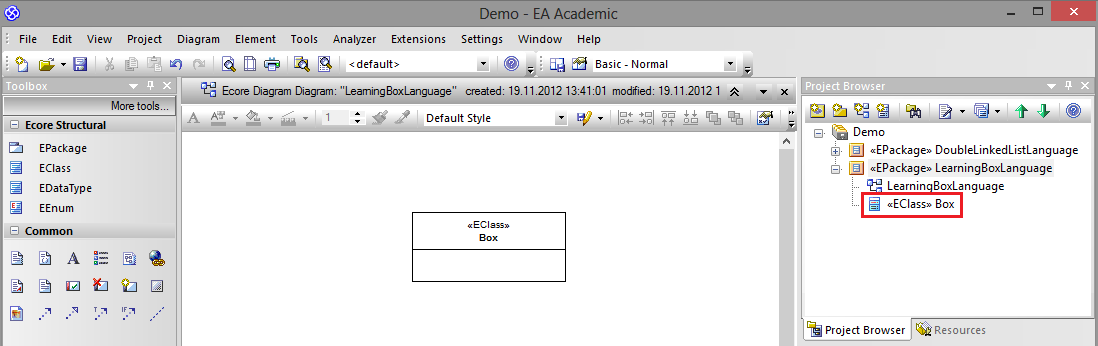
\includegraphics[width=1\textwidth]{ea_afterBoxCreation}
	\caption{State after creating \texttt{Box}}
	\label{fig:eclass_completed}
\end{figure}

\item[$\blacktriangleright$] Now create \texttt{Partition} and \texttt{Card} the same way, until your workspace resembles figure~\ref{fig:all_eclasses}.
These are the main models for our learning box.

\vspace{1cm}

\begin{figure}[htbp]
	\centering
  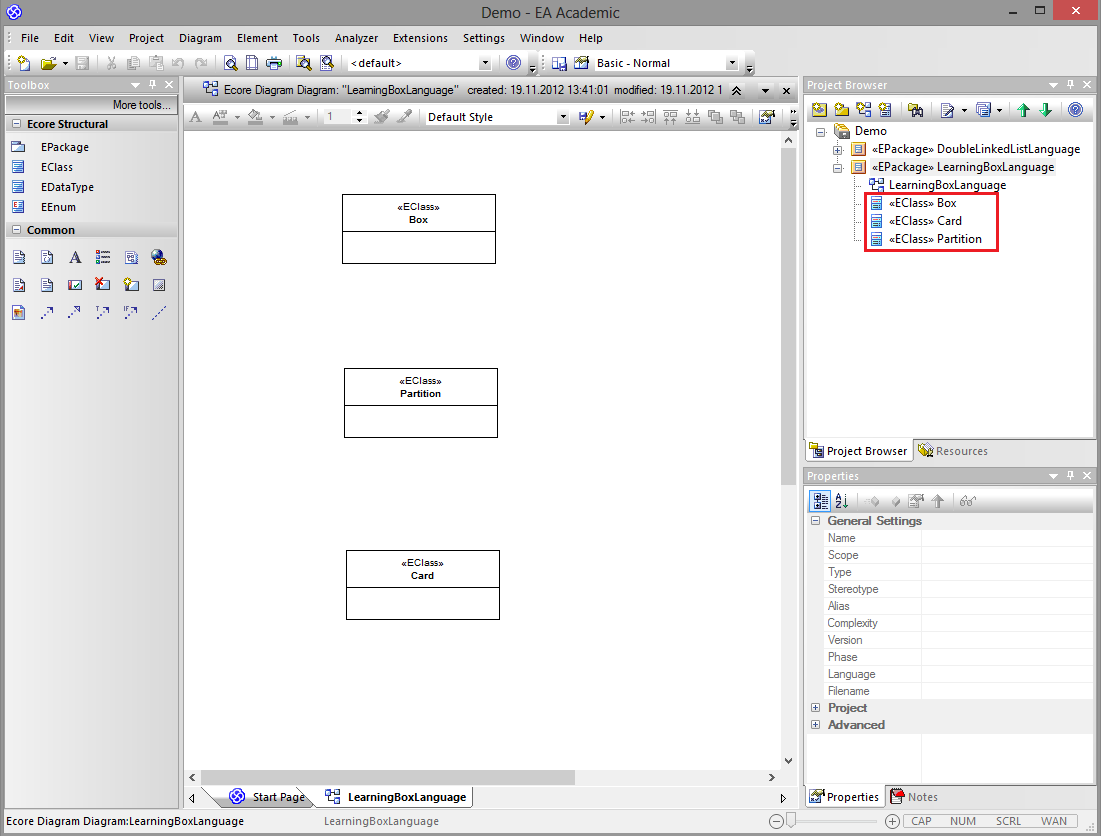
\includegraphics[width=1\textwidth]{EA_createPartitionCard}
	\caption{All classes for our metamodel}
	\label{fig:all_eclasses}
\end{figure}

\vfill
\pagebreak

\item[$\blacktriangleright$] Now choose \texttt{Box}, right-click to call up the context menu and choose ``Features \& Properties/Attributes..'' (Fig.~\ref{fig:attribute}).

\begin{figure}[htbp]
	\centering
  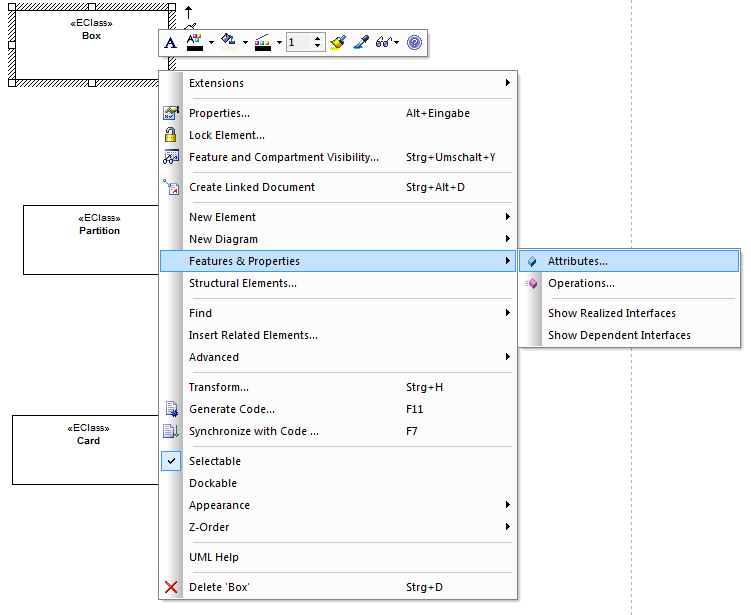
\includegraphics[width=0.6\textwidth]{EA_contextAddAttribute}
	\caption{Context Menu for a class}
	\label{fig:attribute}
\end{figure}
\FloatBarrier

\vspace{0.5cm}

\item[$\blacktriangleright$] In the dialogue that pops-up, enter \texttt{name} as the name of the attribute, choose \texttt{EString} as its type and press \texttt{Save} (Fig.~\ref{fig:attribute_properties}). New attributes for the same class can be added by choosing \texttt{New}.

\vspace{0.5cm}

\begin{figure}[htbp]
	\centering
  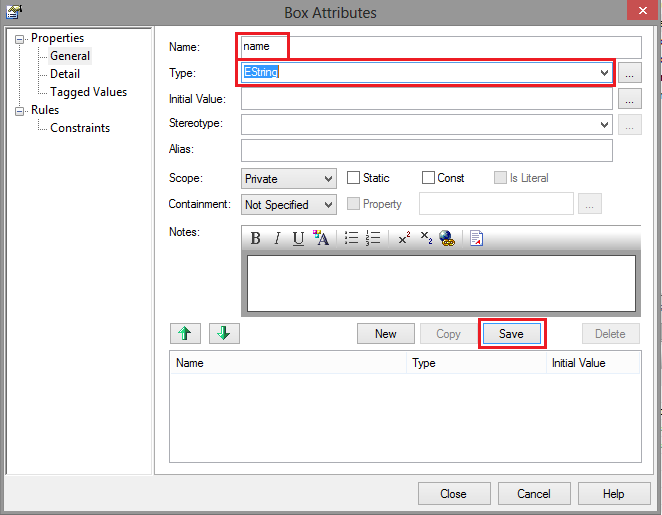
\includegraphics[width=0.6\textwidth]{EA_addingAttributes}
	\caption{Adding attributes to a class}
	\label{fig:attribute_properties}
\end{figure}

\pagebreak

\item[$\blacktriangleright$] Add attributes to all other classes until your workspace resembles figure~\ref{fig:attribute_completed}.

\begin{figure}[htbp]
	\centering
  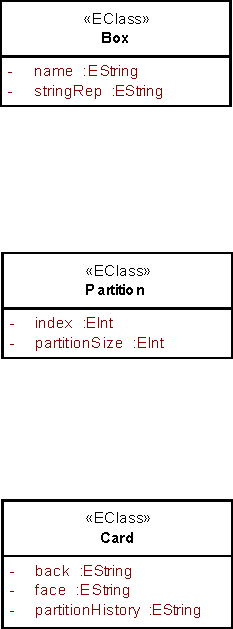
\includegraphics[width=0.25\textwidth]{EA_allAttributes}
	\caption{Main classes with attributes}
	\label{fig:attribute_completed}
\end{figure}
\FloatBarrier


\item[$\blacktriangleright$] A fundamental gesture in EA is \emph{Quick Link}.
Quick Link is used to create links between elements in a context-sensitive manner.
To use Quick Link, choose an element and note the little black arrow in its top-right corner (Fig.~\ref{fig:quicklink}).

\begin{figure}[htbp]
	\centering
  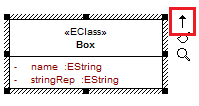
\includegraphics[width=0.4\textwidth]{EA_quickLink}
	\caption{Quick Link is a central gesture in EA}
	\label{fig:quicklink}
\end{figure}
\FloatBarrier

\pagebreak

Click on this black arrow and `pull' to another element you wish to link to.
To start, quick link from \texttt{Box} to \texttt{Partition}.
In the context-menu that pops up, choose \texttt{Create Bidirectional EReference} (Fig.~\ref{fig:ereference}).

\begin{figure}[htbp]
	\centering
  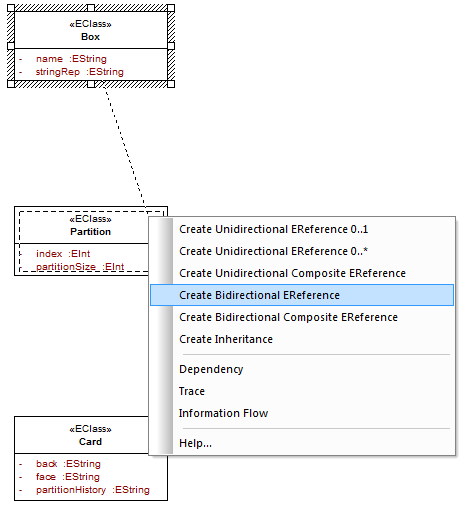
\includegraphics[width=0.5\textwidth]{EA_ereferenceBidirectional}
	\caption{Create a reference via Quick Link}
	\label{fig:ereference}
\end{figure}
\FloatBarrier

\item[$\blacktriangleright$] Double click the reference to invoke a dialogue.
Here you can change the reference direction\footnote{this is particuluary useful if you accidentally click one of the other options while creating the quick link and wish to change it, or if you went backwards from partition to box.} and enter a name. The name will only be used for documentation purposes as it is not relevant for code generation.

\item[$\blacktriangleright$] In the same dialogue, choose \texttt{Target Role} and enter the values in figure~\ref{fig:reference_ends} to set the properties for the ``target'' end of the reference (the \texttt{Box} role). As you can see, the default target is set to the class you linked \emph{from}, and the default source is the class you linked \emph{to}. If you decided to ignore the instructions, and went from \texttt{Partition} to \texttt{Box}, the only difference between the references are the titles - the following information will still be the same! In this window, it's important not to forget to check and modify the \texttt{Role}, \texttt{Navigability}, \texttt{Multiplicity}, and \texttt{Aggregation} settings for the target.  Repeat the process for the \texttt{Source Role}.

\vspace{0.5cm}

\begin{figure}[htbp]
	\centering
	  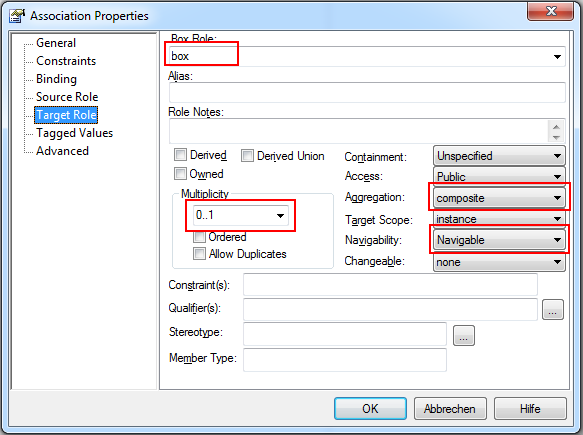
\includegraphics[width=0.73\textwidth]{EA_assocPropsTarget}\\
  \vspace{1cm}
    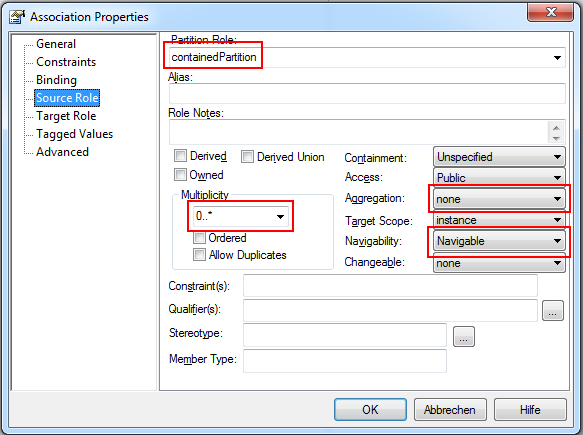
\includegraphics[width=0.73\textwidth]{EA_assocPropsSource}
	\caption{Enter properties for target and source of reference}
	\label{fig:reference_ends}
\end{figure}
\FloatBarrier

\end{itemize}

We reviewed the source and target purposes, but what are the other three options we had to modify? Firstly, navigable ends are mapped to class attributes with getters and setters in Java and therefore \emph{must} have a specified name and  multiplicity for successful code generation. Corresponding values for non-navigable ends can  be regarded as additional documentation and do not have to be specified.

Next, the multiplicity of a reference controls if the relation is mapped to a Java Collection (\texttt{*},  \texttt{1..*}, \texttt{0..*}), or to a single valued class attribute (\texttt{1}, \texttt{0..1}).

Finally, in Ecore, the aggregation values of a reference can either be \texttt{none} or \texttt{com\-po\-site}.
Composite means that the current role is that of a \emph{container} for the opposite role.
In our case for example, \texttt{box} is a container for \texttt{partitions}.\\
This has a series of consequences: (1) every element must have a container, (2) an element cannot be in more than one container at the same time, and (3) a container's contents are deleted together with the container.
Non-composite (\texttt{none}) means that the current role is not that of a container and the rules for containment do not hold (reference is a simple ``pointer'').

\begin{enumerate}

\item[$\blacktriangleright$] If you've done everything right, your workspace should now resemble Fig.~\ref{fig:ereference_completed} with a relation between \texttt{Box} and \texttt{Partition}.

\begin{figure}[htbp]
	\centering
  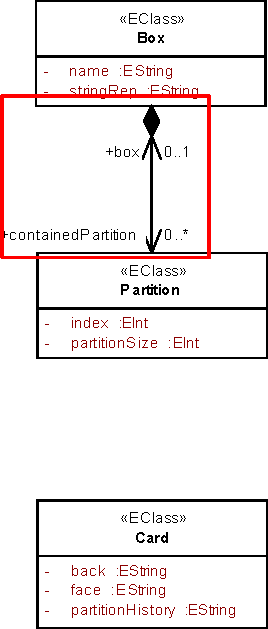
\includegraphics[width=0.3\textwidth]{EA_relationBoxPartition}
	\caption{\texttt{Box} contains \texttt{Partition}s}
	\label{fig:ereference_completed}
\end{figure}
\FloatBarrier


\item[$\blacktriangleright$] Create another bidirectional reference\footnote{To be precise, \emph{all} references in Ecore are actually unidirectional.
A ``bidirectional'' reference in our metamodel is in reality mapped to two \texttt{EReferences} that are opposites of each other.
We however believe it is simpler to handle these pairs as single references and prefer this concise concrete syntax.} between \texttt{Partition} and \texttt{Card}, then two unidirectional self-references for \texttt{Partition} according to Fig.~\ref{fig:ereferences_all}\footnote{If you have difficulties deciphering the role names and other details in this screenshot, please forward to figure~\ref{fig:metamodel_complete} for a better diagram of the metamodel.}.

\begin{figure}[htbp]
	\centering
  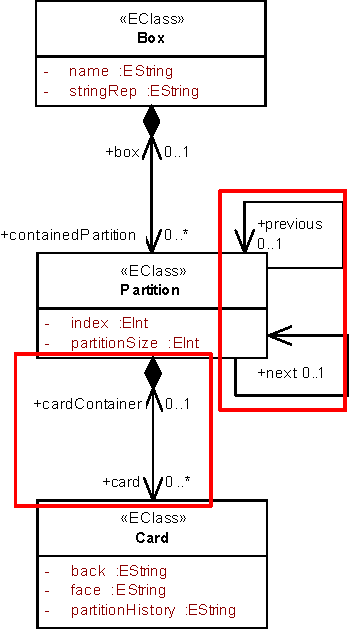
\includegraphics[width=0.5\textwidth]{EA_relationsAll}
	\caption{All relations in our metamodel}
	\label{fig:ereferences_all}
\end{figure}
\end{enumerate}
\FloatBarrier

All of your program attributes and references have now been set up. To see how this would appear in eMoflon's textual syntax, check out figure~\ref{fig:allReferences} and \ref{fig:partitionReferences} in section~\ref{sec:staticConcrete}!

\vfill
\pagebreak

In addition to its static structure, every system has certain dynamic aspects that describe the system's behaviour and how it reacts to external stimulus or evolves over time.
\marginpar{\emph{Dynamic Semantics}}
In a language, these rules that govern the dynamic behaviour of a system are referred to collectively as the \emph{Dynamic Semantics} of the language.
Although these rules can be defined as a set of separate \emph{Model Transformations}, we take a holistic approach and advocate integrating the transformations directly in the metamodel as operations. This naturally fits quite nicely into the OO paradigm.

In the next few steps we shall define the \emph{signatures} of some operations for our learning box. We will use SDMs in Part III of the handbook to \emph{implement} these methods.
\begin{enumerate}
\item[$\blacktriangleright$] Right-click \texttt{Partition} to invoke the context-menu depicted in figure~\ref{fig:add_operation} and choose ``Features \& Properties/Operations..''.

\begin{figure}[htbp]
	\centering
  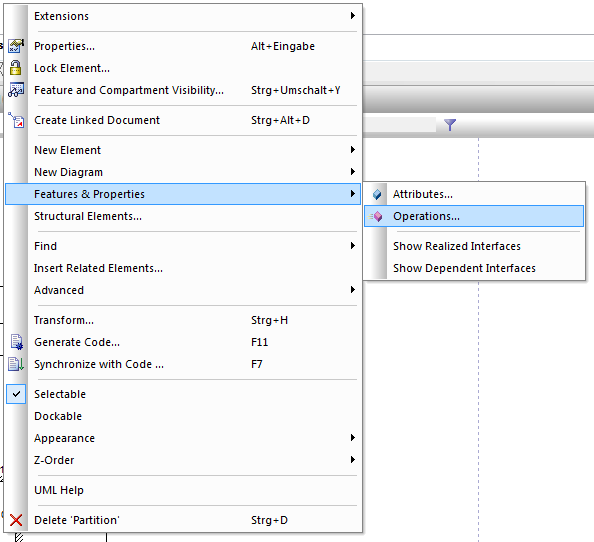
\includegraphics[width=0.7\textwidth]{EA_contextAddOperation}
	\caption{Add an operation}
	\label{fig:add_operation}
\end{figure}
\FloatBarrier

\item[$\blacktriangleright$] In the dialogue that pops-up (Fig.~\ref{fig:operation_properties}), enter \texttt{empty} as the \texttt{Name} of the operation, leave the \texttt{Return Type} as \texttt{void}, and press \texttt{Save}.

\begin{figure}[htbp]
	\centering
  	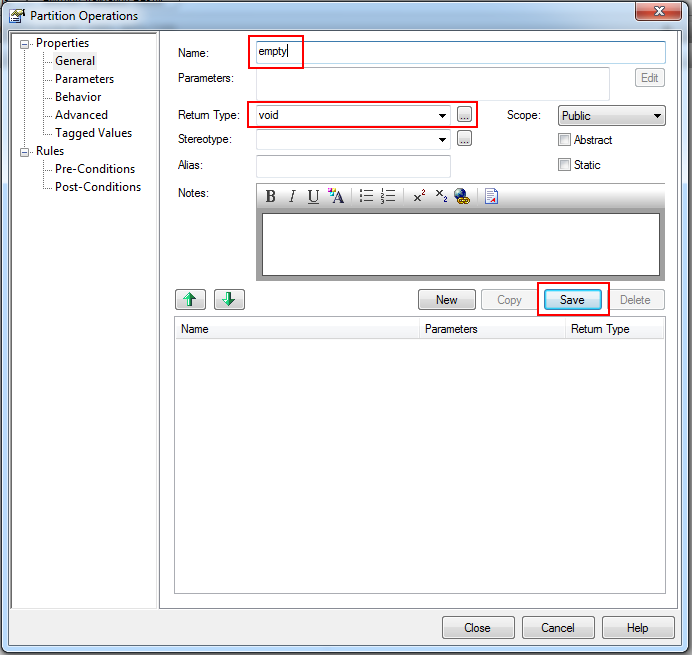
\includegraphics[width=0.5\textwidth]{EA_operationEmpty}
	\caption{Properties for operation}
	\label{fig:operation_properties}
\end{figure}
\FloatBarrier

\item[$\blacktriangleright$] In the same dialogue, press \texttt{New} to add further operations and enter the values in figure~\ref{fig:operation_parameters}.  Parameters can be added by pressing \texttt{Edit}\footnote{You must save the operation before this option will become active.} and entering the name and choosing the type of each parameter in a separate dialogue.

\begin{figure}[htbp]
	\centering
  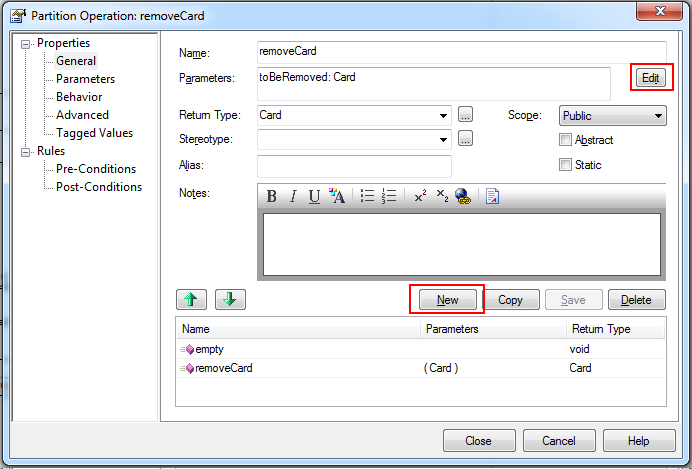
\includegraphics[width=0.9\textwidth]{EA_operationRemoveCard}
	\caption{Parameters and Return Type}
	\label{fig:operation_parameters}
\end{figure}
\FloatBarrier

\vfill
\pagebreak

\item[$\blacktriangleright$] Repeat the process for the \texttt{check} operation in figure~\ref{fig:operation_partition}.
Notice that the \texttt{Return Type} can be chosen via the drop-down menu for primitives (e.g. \texttt{EBoolean}), or via the `\texttt{\ldots}' button (indicated in Fig.~\ref{fig:operation_parameters}) for types you've established in the metamodel (e.g. \texttt{Card}).
\end{enumerate}

\vspace{-.5cm}
\begin{quote}
$\textbf{Please note:}$ Non-primitive types \emph{must} be chosen via the `\texttt{\ldots}' button. It allows you to browse for the corresponding elements in your project. Just typing them won't work!
\end{quote}


\begin{figure}[htbp]
	\centering
  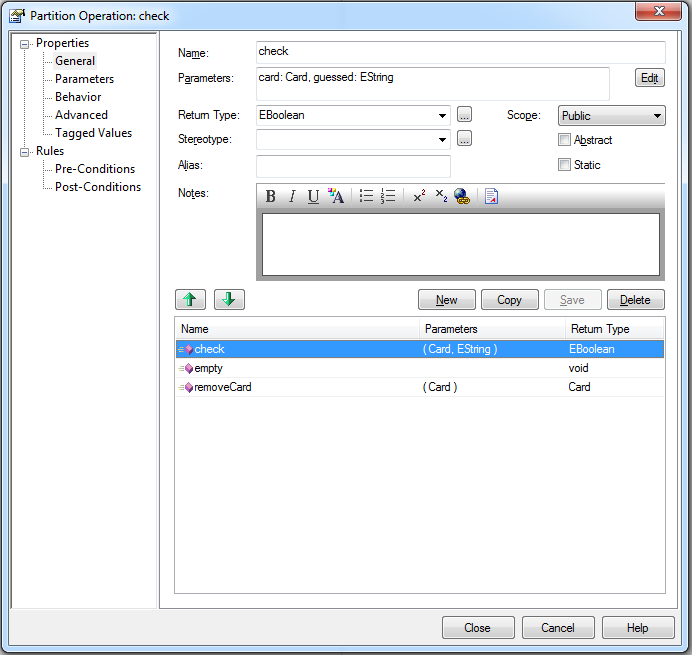
\includegraphics[width=0.9\textwidth]{EA_operationCheck}
	\caption{All operations in \texttt{Partition}}
	\label{fig:operation_partition}
\end{figure}

If you've done everything right, your dialogue should now contain three methods: \texttt{check}, \texttt{empty}, and \texttt{removeCard}, each with corresponding parameters and return types as in Fig.~\ref{fig:operation_partition}.

Add all operations analogously for \texttt{Box} and \texttt{Card}, so that your metamodel closely resembles figure~\ref{fig:metamodel_complete}.

\begin{figure}[htbp]
	\centering
  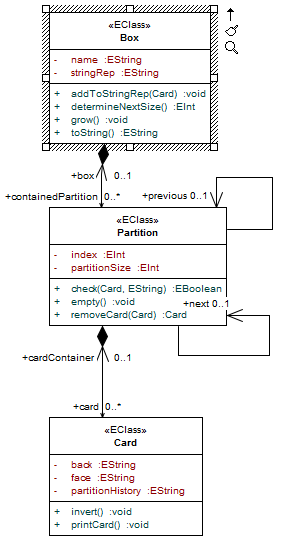
\includegraphics[width=0.7\textwidth]{EA_metamodelComplete.png}
	\caption[Complete metamodel for our learning box.]{Complete metamodel for our learning box \\ \emph{\small Please note that names of parameters may not be displayed by default in EA.}}
	\label{fig:metamodel_complete}
\end{figure}

\pagebreak

To see how this complete metamodel is represented in the textual syntax, review figure~\ref{fig:workspaceMethods} in section~\ref{sec:staticConcrete}.

\begin{enumerate}
\item[$\blacktriangleright$] To finish, try to export the metamodel for code generation in Eclipse~\footnote{if problems occur during the following steps, we recommend reading \texttt{Part VI: Micellaneous}. This might help you to find your mistakes}. Right-click on \texttt{LearningBoxLanguage} and choose ``Extensions/MOFLON::Ecore Addin/Export Selection to Workspace''.
Then switch to your Eclipse work\-space and refresh the metamodel workingset. Alternatively, you can activate eMoflon's add-in window by going to ``Extensions/Add-in Windows,'' and pressing \texttt{All} in the \texttt{Export} box.
\end{enumerate}


If you've done everything correctly, a new project \texttt{LearningBoxLanguage} should be created in the \texttt{Demo} working set within your eclipse workspace.
If this is not the case, please ensure that your metamodel is identical with figure~\ref{fig:metamodel_complete}.

If you believe everything is correct and things still don't work, feel free to contact us at \href{mailto:contact@moflon.org}{contact@moflon.org}.

If code is generated successfully, take a look at all the stuff that's been generated under \texttt{/gen}. Especially look at the the default implementation for all methods who throw an  \texttt{OperationNotSupported} exception.
We shall see later in the handbook that the Eclipse Modeling Foundation's (EMF) code generator actually supports injecting hand-written implementations of methods into generated methods and classes.
With eMoflon however, we can also model a large part of the dynamic semantics, and only need to implement small helper methods, such as string manipulation by hand.

\fancyfoot[R]{ $\triangleright$ \hyperlink{static review}{Next task} }